% THIS IS SIGPROC-SP.TEX - VERSION 3.1
% WORKS WITH V3.2SP OF ACM_PROC_ARTICLE-SP.CLS
% APRIL 2009
%
% It is an example file showing how to use the 'acm_proc_article-sp.cls' V3.2SP
% LaTeX2e document class file for Conference Proceedings submissions.
% ----------------------------------------------------------------------------------------------------------------
% This .tex file (and associated .cls V3.2SP) *DOES NOT* produce:
%       1) The Permission Statement
%       2) The Conference (location) Info information
%       3) The Copyright Line with ACM data
%       4) Page numbering
% ---------------------------------------------------------------------------------------------------------------
% It is an example which *does* use the .bib file (from which the .bbl file
% is produced).
% REMEMBER HOWEVER: After having produced the .bbl file,
% and prior to final submission,
% you need to 'insert'  your .bbl file into your source .tex file so as to provide
% ONE 'self-contained' source file.
%
% Questions regarding SIGS should be sent to
% Adrienne Griscti ---> griscti@acm.org
%
% Questions/suggestions regarding the guidelines, .tex and .cls files, etc. to
% Gerald Murray ---> murray@hq.acm.org
%
% For tracking purposes - this is V3.1SP - APRIL 2009

\documentclass{acm_proc_article-sp}

\usepackage{amsmath}
\usepackage{caption}
\usepackage{float}
\usepackage{graphicx} % support the \includegraphics command and options
% for osx:
% \usepackage[backend=biber]{biblatex} % use biber command to regenerate references
% for ubuntu:
\usepackage{biblatex}
\usepackage{subcaption}

\renewcommand{\bibfont}{\footnotesize}
%\pagenumbering{gobble}
\usepackage{hyperref}
\addbibresource{report.bib}


\begin{document}

\title{Parallelised Pose Estimation for Automated Landing}
\subtitle{CS267: Project Report}
%
% You need the command \numberofauthors to handle the 'placement
% and alignment' of the authors beneath the title.
%
% For aesthetic reasons, we recommend 'three authors at a time'
% i.e. three 'name/affiliation blocks' be placed beneath the title.
%
% NOTE: You are NOT restricted in how many 'rows' of
% "name/affiliations" may appear. We just ask that you restrict
% the number of 'columns' to three.
%
% Because of the available 'opening page real-estate'
% we ask you to refrain from putting more than six authors
% (two rows with three columns) beneath the article title.
% More than six makes the first-page appear very cluttered indeed.
%
% Use the \alignauthor commands to handle the names
% and affiliations for an 'aesthetic maximum' of six authors.
% Add names, affiliations, addresses for
% the seventh etc. author(s) as the argument for the
% \additionalauthors command.
% These 'additional authors' will be output/set for you
% without further effort on your part as the last section in
% the body of your article BEFORE References or any Appendices.

\numberofauthors{3} %  in this sample file, there are a *total*
% of EIGHT authors. SIX appear on the 'first-page' (for formatting
% reasons) and the remaining two appear in the \additionalauthors section.
%
\author{
% You can go ahead and credit any number of authors here,
% e.g. one 'row of three' or two rows (consisting of one row of three
% and a second row of one, two or three).
%
% The command \alignauthor (no curly braces needed) should
% precede each author name, affiliation/snail-mail address and
% e-mail address. Additionally, tag each line of
% affiliation/address with \affaddr, and tag the
% e-mail address with \email.
%
% 1st. author
\alignauthor
Sunil Shah\\
       \email{sunil.shah@berkeley.edu}
% 2nd. author
\alignauthor
Nahush Bhanage\\
       \email{nahush@berkeley.edu}
% 3rd. author
\alignauthor 
Hoang Nguyen\\
       \email{hoanghw@berkeley.edu}
}
% There's nothing stopping you putting the seventh, eighth, etc.
% author on the opening page (as the 'third row') but we ask,
% for aesthetic reasons that you place these 'additional authors'
% in the \additional authors block, viz..}
\date{12 May 2014}
% Just remember to make sure that the TOTAL number of authors
% is the number that will appear on the first page PLUS the
% number that will appear in the \additionalauthors section.

\maketitle
\begin{abstract}
Current approaches for automated landing of unmanned aerial vehicles (UAVs) are
based on GPS localization, which we show is quite inaccurate. We optimise a previously implemented computer vision based pose estimation algorithm to run in real time on a low cost open source embedded computer.
\end{abstract}

% A category with the (minimum) three required fields
\category{H.4}{Information Systems Applications}{Miscellaneous}
%A category including the fourth, optional field follows...
\category{D.2.8}{Software Engineering}{Metrics}[complexity measures, performance measures]

\terms{Theory}

\keywords{ACM proceedings, \LaTeX, text tagging} % NOT required for Proceedings

%%%%%%%%%%%%%%%%%%%%%%%%%%%%%%%%%%%%%%%%%%%%%%%%%%%%%%%%%%%%%%%%%%%%%%%%%%%%%%
\section{Introduction}



%%%%%%%%%%%%%%%%%%%%%%%%%%%%%%%%%%%%%%%%%%%%%%%%%%%%%%%%%%%%%%%%%%%%%%%%%%%%%%
\section{Prior Work}


%%%%%%%%%%%%%%%%%%%%%%%%%%%%%%%%%%%%%%%%%%%%%%%%%%%%%%%%%%%%%%%%%%%%%%%%%%%%%%
\section{System Description}

\subsection{Hardware Architecture}
% Autopilot
% Embedded computer
% Peripheral hardware
% Architecture diagram

\subsection{Software Design}
% Operating system and library setup


\subsection{Automated Landing}

\subsubsection{Landing Pad Design}
\subsubsection{Algorithm Overview}
\paragraph{Corner Detection}
\paragraph{Pose Estimation}

\subsubsection{Real-time Control}

%%%%%%%%%%%%%%%%%%%%%%%%%%%%%%%%%%%%%%%%%%%%%%%%%%%%%%%%%%%%%%%%%%%%%%%%%%%%%%
\section{Approach}
% List of optimisations

\subsection{Profiling}



\subsection{Compiler Optimisations}
%% PARALLELISM HERE

\subsection{Library Optimisations}
%% PARALLELISM HERE

\subsection{Single-threaded Optimisations}

\subsection{Multi-threaded Optimisations}


%%%%%%%%%%%%%%%%%%%%%%%%%%%%%%%%%%%%%%%%%%%%%%%%%%%%%%%%%%%%%%%%%%%%%%%%%%%%%%
\section{Results}

\subsection{Benchmarking Methodology}

\subsection{Maximum Performance}

\subsection{Performance of Naive Implementation}

\subsection{Performance of Naive Implementation with Optimised Libraries}

\subsection{Performance of Single-threaded Optimised Implementation}

\subsection{Performance of Multi-threaded Optimised Implementation}

\subsection{Performance of Single-threaded Optimised Implementation (2)}

\subsection{Performance Summary}


%%%%%%%%%%%%%%%%%%%%%%%%%%%%%%%%%%%%%%%%%%%%%%%%%%%%%%%%%%%%%%%%%%%%%%%%%%%%%%
\section{Conclusion}


\begin{figure}[h!]
\centering
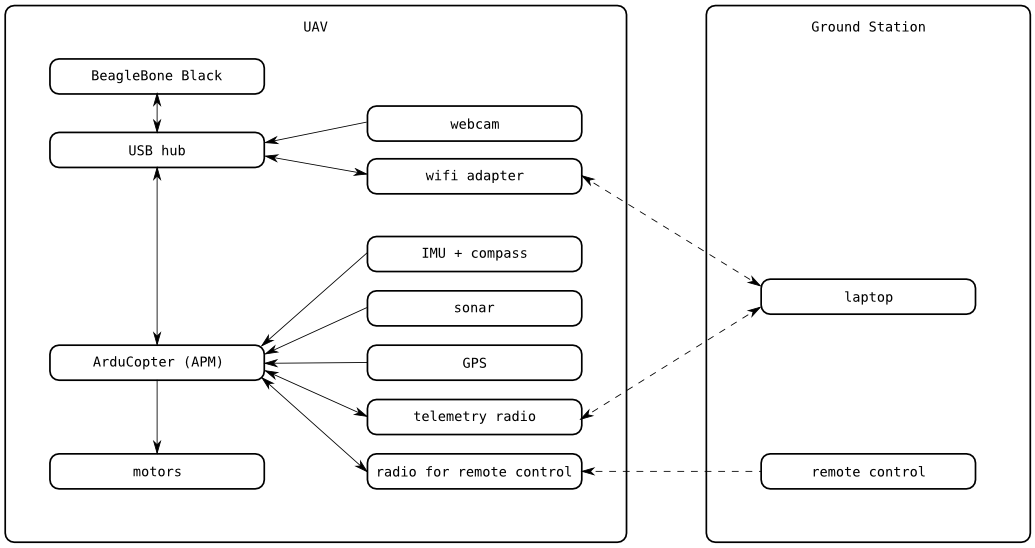
\includegraphics[width=0.9\textwidth]{images/architecture.png}
\caption{
    Architecture of our automated landing system. We use inexpensive
    off-the-shelf hardware. The laptop and remote control are for
    monitoring and emergency takeover by a human pilot. All the
    computation is performed onboard the UAV.
}
\label{fig:hardware-arch}
\end{figure}

\begin{figure}[h!]
\centering
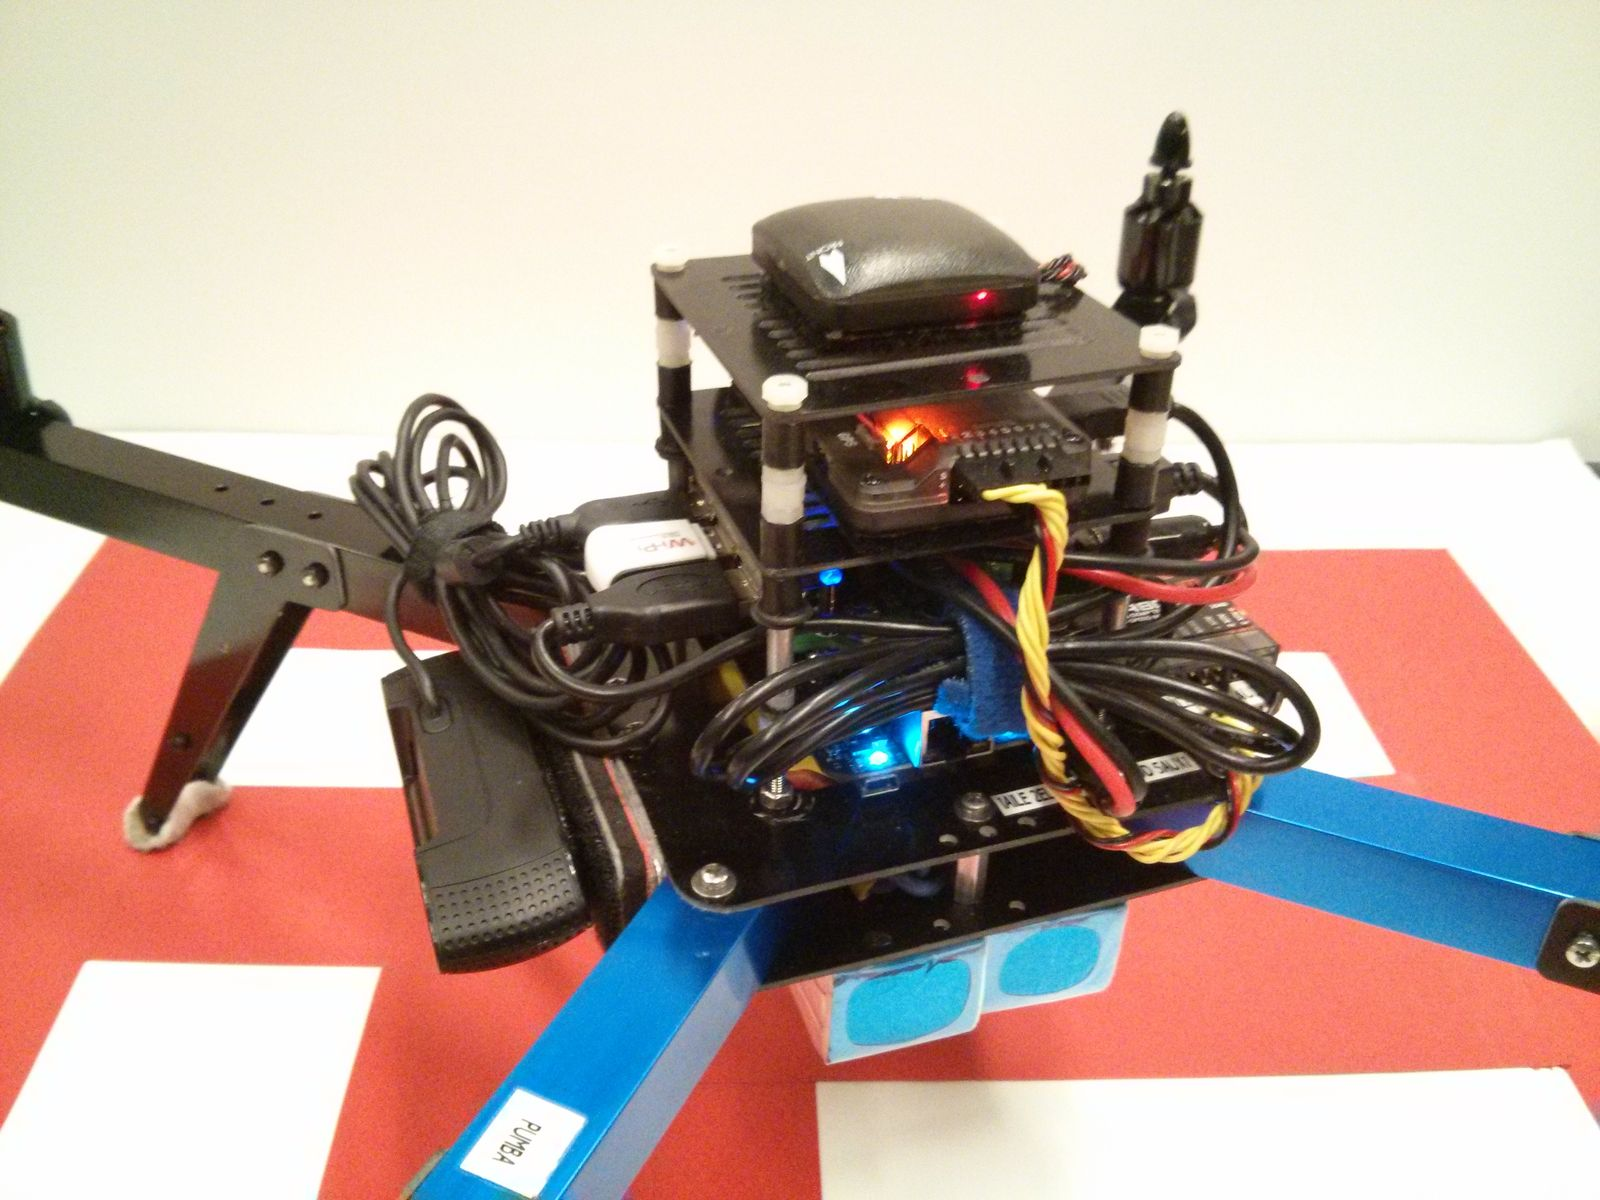
\includegraphics[width=0.85\textwidth]{images/hardware.jpg}
\caption{
    Our hardware stack fully assembled. From bottom to top: batteries,
    BeagleBone embedded computer, USB hub with Wi-Fi adapter, 3D
    Robotics autopilot with embedded sensors, GPS module. The
    webcam is on the left, and the radio for the remote control is on
    the right. Total weight excluding batteries is 1.35 kg.
}
\label{fig:hardware-photo}
\end{figure}

\begin{figure*}[h]
    \centering
    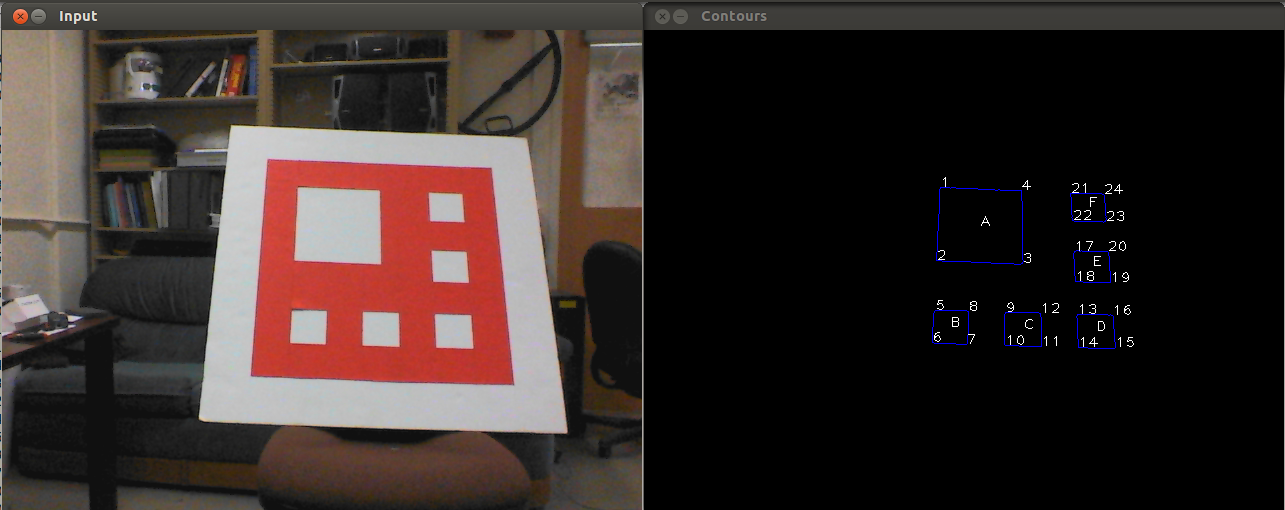
\includegraphics[width=\textwidth]{images/corners.png}
    \caption{
        Left: Design of our landing platform.
        Right: Output of the corner detector (24 points, in order).
    }
    \label{fig:corners}
\end{figure*}

\begin{figure}
    \begin{minipage}{0.5\textwidth}
        \centering
        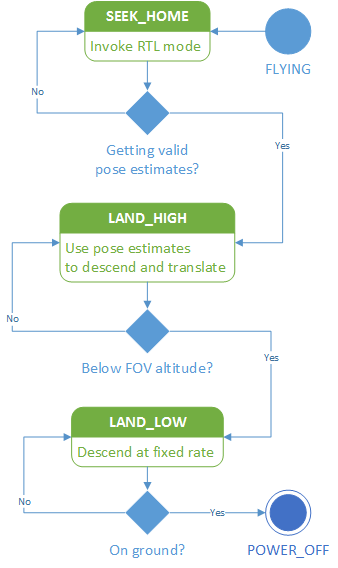
\includegraphics[width=0.9\linewidth]{images/statediagram.png}
        \caption{State diagram of our landing controller.}
        \label{fig:statediagram}
    \end{minipage}% this comment necessary, otherwise extra newline treated as space
    \begin{minipage}{0.5\textwidth}
        \centering
        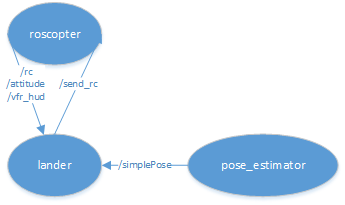
\includegraphics[width=0.9\linewidth]{images/rosnodes.png}
        \caption{ROS nodes and topics for exchanging messages.}
        \label{fig:rosnodes}
        \vspace{2cm}
        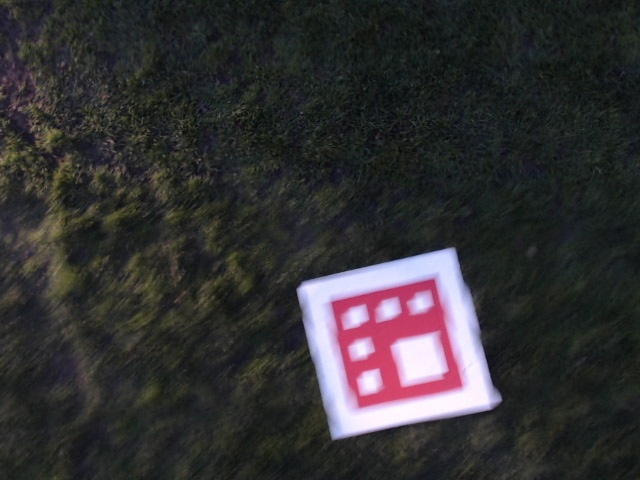
\includegraphics[width=0.9\linewidth]{images/badimage.jpg}
        \caption{An image where pose estimation fails.}
        \label{fig:badimage}
    \end{minipage}
\end{figure}


%
% The following two commands are all you need in the
% initial runs of your .tex file to
% produce the bibliography for the citations in your paper.
%\bibliographystyle{abbrv}
%\bibliography{sigproc}  % sigproc.bib is the name of the Bibliography in this case
\printbibliography
% You must have a proper ".bib" file
%  and remember to run:
% latex bibtex latex latex
% to resolve all references
%
% ACM needs 'a single self-contained file'!
%
%APPENDICES are optional
%\balancecolumns
\appendix
%Appendix A
\end{document}
